% M05_confinement_theory.tex -- quantum confinement, effective masses, non-parabolicity and band alignment in thin
% slabs, tested against the computed crystalline series. Analysis: tools/confinement_analysis.py ->
% evidence/derived/confinement_analysis.json (FACT-027..029a); figure tools/fig_confinement_models.py.
\chapter{Quantum confinement, effective masses and band alignment in thin slabs}
\label{ch:mono-confinement-theory}

The device model needs three thickness laws from first principles: how far the conduction-band edge rises ($\dEc$),
how heavy the electrons become ($\mstar$), and how the effective density of states changes ($\Nc$). This chapter
derives what simple band-structure models predict for these quantities and tests the predictions against the computed
crystalline slab series of \cref{ch:dft} and \cref{sec:mono-dft-thin}. The tests use only computed numbers and contain
no fit to device data. They show which parts of the computed thickness dependence follow from bulk band structure
alone and which do not, and that distinction decides how much of the first-principles input the device model can
trust (\cref{ch:mono-multiscale}).

% =====================================================================================================================
\section{The envelope-function picture}
\label{sec:mono-conf-ema}

Near a band minimum at $\Gamma$ with energy $E_c$ and an isotropic mass $m_b$, a state of a slowly varying confining
potential $U(z)$ can be written as $\psi = F(z)e^{i\vk_\parallel\cdot\vr_\parallel}u_{c,0}(\vr)$, where $u_{c,0}$ is the
lattice-periodic band-edge function and $F$ the envelope. To lowest order in $k\cdot p$ the envelope obeys
\begin{equation}
\Big[-\frac{\hbar^2}{2m_b}\frac{d^2}{dz^2} + U(z)\Big]F_n = \Big(E - E_c - \frac{\hbar^2k_\parallel^2}{2m_b}\Big)F_n ,
\label{eq:mono-conf-envelope}
\end{equation}
with continuity of $F$ and of $F'/m$ at interfaces \citep{Bastard1981}. For a well of width $t$ with infinite barriers,
$F_n = \sin(n\pi z/t)$ and
\begin{equation}
E_n - E_c = \frac{\hbar^2\pi^2n^2}{2m_bt^2} = \frac{0.376\,\mathrm{eV\,nm^2}}{(m_b/m_0)\,t^2}\,n^2 .
\label{eq:mono-conf-inf}
\end{equation}
This predicts $\dEc \propto t^{-2}$. With the computed bulk band-edge mass $m_b = 0.1541\,m_0$ \fact{004} and $t$ equal
to the H--H thickness, it gives 0.634~eV at 1.962~nm, 2.3 times the computed $\dEc = 0.281$~eV.

\paragraph{Validity.} \Cref{eq:mono-conf-envelope} assumes that $F$ varies slowly on the scale of the unit cell. The
bixbyite lattice constant is 1.03~nm; the 1~nm film is thinner than one cell and the 2~nm film spans two. The envelope
picture is therefore not justified a priori for any film of this study, and it should be read as a parametrisation to
be tested, not as a derivation. A finite barrier does not rescue it: the vacuum barrier is the electron affinity, about
4~eV, and the decay length of a free electron into it, $\hbar/\sqrt{2m_0\cdot4\,\mathrm{eV}}\approx0.1$~nm, is far too
small to explain the factor 2.3.

\section{Non-parabolicity}
\label{sec:mono-conf-kane}

In a two-band $k\cdot p$ model of a direct-gap semiconductor with gap $\Eg$ and interband matrix element expressed by
the energy $E_P$, the conduction band obeys, to leading order, the Kane dispersion \citep{Kane1957}
\begin{equation}
E(1+\alpha E) = \frac{\hbar^2k^2}{2m_b}, \qquad \frac{m_0}{m_b} = 1 + \frac{E_P}{\Eg},\qquad
\alpha = \frac{1}{\Eg}\Big(1-\frac{m_b}{m_0}\Big)^2 ,
\label{eq:mono-conf-kane}
\end{equation}
with $E$ measured from the band minimum. The computed bulk band of \InO{} along [100], [110] and [111] follows the
first relation with $m_b = 0.1541\,m_0$ and $\alpha = 0.58$~eV$^{-1}$ (0.55--0.63 over directions and windows;
isotropic within 0.2\,\%) up to 0.45~eV above the minimum \fact{004} \fact{005}. The two-band expression for $\alpha$
with the PBE gap would give 0.81~eV$^{-1}$, so remote bands reduce the non-parabolicity; $\alpha$ is therefore taken
from the fit, not from \cref{eq:mono-conf-kane}.

\paragraph{The gap does not set the mass.} The second relation of \cref{eq:mono-conf-kane} with the PBE gap and mass
gives $E_P = 4.9$~eV. Kept fixed, this $E_P$ would make the mass $0.30\,m_0$ at the HSE06 gap of 2.1~eV, whereas the
HSE06 estimates are $0.159$--$0.193\,m_0$ \claim{C039}; and the measured band-edge mass of $0.208\pm0.006\,m_0$
\citep[p.~225102-1]{Stokey2021} together with a fundamental gap near 2.8~eV would require $E_P \approx 11$~eV (the
literature values of the mass span 0.13--0.55~$m_0$, \citealp[p.~225102-2]{Stokey2021}). The conduction-band mass of
\InO{} is therefore not controlled by the gap in the two-band way, which is consistent with PBE giving a mass 26\,\%
below that measurement while its gap is low by a factor of three. Masses have to be computed;
they cannot be scaled from gaps.

\section{Confined subbands in a non-parabolic band}
\label{sec:mono-conf-subband}

Quantising the out-of-plane wave vector, $k_z = n\pi/t$, in the Kane dispersion and keeping the in-plane part gives,
for the subband $n$,
\begin{equation}
E(1+\alpha E) = \varepsilon_n + \frac{\hbar^2k_\parallel^2}{2m_b},\qquad \varepsilon_n = \frac{\hbar^2\pi^2n^2}{2m_bt^2} .
\label{eq:mono-conf-sub}
\end{equation}
Three consequences follow, each without free parameters.

\paragraph{(i) Subband energy and its exponent.} At $k_\parallel = 0$, $E_n = [-1+(1+4\alpha\varepsilon_n)^{1/2}]/(2\alpha)$.
Since $\varepsilon_n \propto t^{-2}$, differentiating $E_n(1+\alpha E_n)$ gives the local power-law exponent
\begin{equation}
p(E) \equiv -\frac{d\ln E}{d\ln t} = 2\,\frac{1+\alpha E}{1+2\alpha E} ,
\label{eq:mono-conf-p}
\end{equation}
which falls from 2 (parabolic, $\alpha E \ll 1$) towards 1 (strongly non-parabolic). At the computed shifts it is 1.75
at 2~nm and 1.50 at 1~nm.

\paragraph{(ii) In-plane mass of the confined subband.} Differentiating \cref{eq:mono-conf-sub} with respect to
$k_\parallel$ at $k_\parallel = 0$ gives $(1+2\alpha E_n)\,dE = \hbar^2k_\parallel\,dk_\parallel/m_b$, so the in-plane
band-edge mass of the subband is
\begin{equation}
m_\parallel = m_b\,(1 + 2\alpha E_n) ,
\label{eq:mono-conf-mpar}
\end{equation}
and expanding to the next order gives an in-plane non-parabolicity $\alpha_\parallel = \alpha/(1+2\alpha E_n)$. The
mass increase of a confined film is, in this picture, the bulk band's non-parabolicity probed at the energy $E_n$.

\paragraph{(iii) Subband spacing.} $E_2-E_1$ is smaller than the parabolic $3E_1$; the ratio falls as the confinement
grows (computed at $\Gamma$: 2.56 at 2~nm and 1.77 at 1~nm, from the logged second levels 0.72 and 1.50~eV above the
minimum).

\section{Test against the computed films}
\label{sec:mono-conf-test}

\Cref{eq:mono-conf-mpar} can be tested directly: with the computed $\dEc$ of each film in place of $E_1$ and the bulk
$m_b$ and $\alpha$, it predicts the in-plane mass with no adjustable quantity. \Cref{tab:mono-conf-test} and
\cref{fig:mono-conf-models} compare the predictions with the computed band-edge masses.

\begin{table}[htbp]\centering\small
\caption{Kane predictions against the computed crystalline films (PBE). $m_\parallel$: in-plane band-edge mass
(computed: 2-D DOS mass, 10-point Kane basis); predicted from \cref{eq:mono-conf-mpar} with $m_b = 0.1541\,m_0$,
$\alpha = 0.58$~eV$^{-1}$ and the computed $\dEc$ (range for $\alpha = 0.55$--0.63 in brackets). $t_{\mathrm{eff}}$:
box width for which the bulk Kane band gives the computed $\dEc$. \fact{027}}
\label{tab:mono-conf-test}
\begin{tabular}{lcccccc}\toprule
$\tHH$ (nm) & $\dEc$ (eV) & $m_\parallel$ computed & $m_\parallel$ predicted & $\alpha_\parallel$ computed / predicted & $t_{\mathrm{eff}}/\tHH$ & $p(E)$ \\\midrule
0.461$^a$ & 1.585 & 0.443 & 0.437 [0.423--0.462] & 0.24 / 0.20 & 1.94 & 1.35 \\
0.695$^b$ & 1.059 & 0.337 & 0.343 [0.334--0.360] & 0.31 / 0.26 & 1.72 & 1.45 \\
0.930 & 0.848 & 0.279 & 0.306 [0.298--0.319] & 0.36 / 0.29 & 1.49 & 1.50 \\
1.962 & 0.281 & 0.203 & 0.204 [0.202--0.208] & 0.47 / 0.44 & 1.39 & 1.75 \\\bottomrule
\multicolumn{7}{l}{\footnotesize $^a$ In$_8$(OH)$_{24}$, outside the termination model. $^b$ Polar; $\dEc$ carries a
reference-choice sensitivity of $\pm0.17$~eV.}
\end{tabular}
\end{table}

\begin{figure}[htbp]\centering
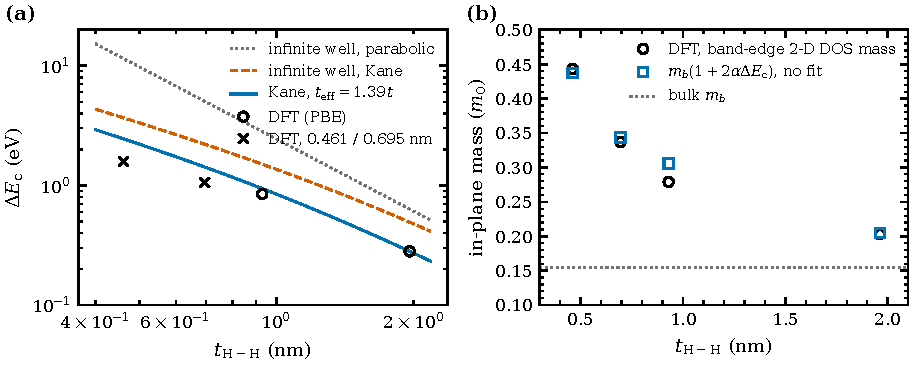
\includegraphics[width=\linewidth]{mono_confinement_models}
\caption{Computed crystalline \InO{}(001) films (PBE) against confinement models. (a) Conduction-band shift $\dEc$ against
the H--H thickness: computed points (circles; crosses for the 0.461~nm In$_8$(OH)$_{24}$ and the polar 0.695~nm film);
an infinite parabolic well with the bulk mass and $t = \tHH$ (dotted); the same with the bulk Kane non-parabolicity
(dashed); a Kane band with a box width $1.39\,\tHH$, the factor that reproduces the 2~nm point (solid). (b) In-plane
band-edge mass: computed (circles) against $m_b(1+2\alpha\dEc)$ evaluated with the computed $\dEc$, with no fitted
quantity (squares); dotted: bulk $m_b$. Source: \file{research_monograph/tools/fig_confinement_models.py}.}
\label{fig:mono-conf-models}
\end{figure}

\paragraph{What the test shows.}
\begin{enumerate}
\item \emph{The mass increase is a bulk band-structure effect.} The no-fit Kane relation reproduces the computed
in-plane masses within 2\,\% at 0.461, 0.695 and 1.962~nm and overestimates the 0.930~nm mass by 10\,\% \fact{027}. The
increase of the mass with confinement is therefore, to this accuracy, the bulk non-parabolicity probed at the energy of
the confined subband, not a surface or termination effect. (The 1~nm deviation remains even with the two-step value
of $\dEc$, 0.819~eV, which gives 0.300~$m_0$.) The predicted in-plane non-parabolicities are 6--19\,\% below the
computed ones, with the right trend.
\item \emph{The shift itself is not a box with a fixed width.} No single box width reproduces $\dEc$ at all
thicknesses: the effective width that the bulk Kane band needs grows from $1.39\,\tHH$ at 2~nm to $1.49\,\tHH$ at 1~nm
(and $1.72$--$1.94\,\tHH$ for the two sub-nanometre films). Equivalently, with a box width proportional to $t$ fixed at
2~nm, the Kane band predicts $\dEc(1~\mathrm{nm}) = 0.94$~eV against the computed 0.848~eV, and an exponent of 1.62
between 1 and 2~nm against the computed 1.48 \fact{028}. The computed band flattens more than the bulk Kane band at
large $k_z$, which is expected because the Kane fit was made only up to 0.45~eV above the minimum.
\item \emph{Consequence for the device model.} The fitted mass law $\Delta m = 0.1145\,t^{-1.2755}$ and the fitted
$\dEc$ law are not independent: within 10\,\% the first follows from the second through \cref{eq:mono-conf-mpar}. A
device model that uses both laws carries one independent first-principles input, not two (\cref{ch:mono-multiscale}).
\end{enumerate}

\section{The valence band and the partition of the gap opening}
\label{sec:mono-conf-partition}

In the envelope picture the opening divides between the bands in inverse proportion to the masses in the confinement
direction: $\dEc/\Delta\Eg = m_h/(m_e+m_h)$ for single bands. The \InO{} valence-band top is a heavy, three-fold
degenerate manifold with directional masses near $\Gamma$ of 3.2--7.9~$m_0$ (band 174) and heavier \claim{C040}.
Single-band EMA therefore predicts that 95--99\,\% of the opening is in the conduction band and that the valence-band
top moves down by only $-0.014$~eV at 2~nm and $-0.041$~eV at 1~nm (for $m_h = 3.2\,m_0$) \fact{029}. The computed
shares are 0.84 (2~nm) and 0.94 (1~nm), and the computed valence shifts are $-0.054$ and $-0.052$~eV: almost
thickness-independent instead of scaling with $\dEc$.

The difference, about 40~meV at 2~nm, is of the same size as the spread between alignment routes: at 2~nm the
two-step and double-average routes give $-0.054$ and $-0.049$~eV, and at 1~nm the two-step route gives $-0.081$~eV and
the EA/IP route $-0.052$~eV (\cref{tab:dft-partition}). The computed thickness-independent valence shift is therefore
not a resolved physical effect (\prov{inferred}). Possible origins, none tested, are a termination-induced potential
offset inside the film that the macroscopic average does not remove, the coupling of the three degenerate valence bands
under confinement, and the small in-plane strain of the films. For the device model the consequence is limited: the
model uses only $\dEc$ (through the electron affinity) and the gap; a constant $\Delta E_{\mathrm{v}}\approx-0.05$~eV
changes the gap but not the electron barrier.

\paragraph{Why the gap law has a smaller exponent than the conduction-band law.} Between 1 and 2~nm, $\dEc$ scales
with an exponent of 1.48 and $\Delta\Eg$ with 1.32 \fact{028}. Since $\Delta\Eg = \dEc - \Delta E_{\mathrm{v}}$ and
$\Delta E_{\mathrm{v}}$ is nearly constant ($-0.053$~eV), the gap carries a thickness-independent offset that lowers its
log-slope; $\ln(0.8998/0.3352)/\ln(1.962/0.930) = 1.32$ follows from the two $\dEc$ values plus 0.053~eV. Laws fitted
to $\Delta\Eg$ and to $\dEc$ therefore must not be used interchangeably.

\section{Why the hybrid-functional ratio is close to one}
\label{sec:mono-conf-hse}

HSE06 opens the bulk gap by a factor of 2.3, yet changes the confinement shift of the 1~nm film by only 6--11\,\%
\fact{030}. Two effects compete. HSE06 makes the band heavier (estimates $0.159$--$0.193\,m_0$), which lowers
$\varepsilon_1 \propto 1/m_b$; and a larger gap makes the band less non-parabolic, which raises $E_1$ for a given
$\varepsilon_1$. Scaling $\alpha$ with the inverse gap, as the two-band model suggests ($\alpha_{\mathrm{HSE}} \approx
0.58\times0.889/2.108 = 0.245$~eV$^{-1}$; an assumption), the Kane band gives $r = E_1^{\mathrm{HSE}}/E_1^{\mathrm{PBE}} =
0.99$--1.17 over the HSE06 mass range, which brackets the computed 1.06--1.11 \fact{029a}. The near-cancellation is
therefore expected; it is a plausibility argument, not a derivation of $r$, and it does not justify transferring $r$
from 1~nm to other thicknesses, which the gap-anchoring scheme does as an assumption (\amend{A23}).

\section{Effective densities of states}
\label{sec:mono-conf-dos}

\paragraph{Three dimensions.} For a parabolic band, $\Nc = 2(2\pi m_b\kT/h^2)^{3/2} = 2.509\times10^{19}(m_b/m_0)^{3/2}$\cmcu{}
at 300~K. For the Kane band the density of states is $g(E) \propto [E(1+\alpha E)]^{1/2}(1+2\alpha E)$; to first order in
$\alpha E$ this is $E^{1/2}(1+\tfrac52\alpha E)$, and averaging $E$ over a Boltzmann distribution weighted with $E^{1/2}$
($\langle E\rangle = \tfrac32\kT$) gives
\begin{equation}
\Nc^{\mathrm{Kane}} \approx \Nc\Big(1+\tfrac{15}{4}\alpha\kT\Big) ,
\label{eq:mono-conf-nc3d}
\end{equation}
a factor of 1.056 for $\alpha = 0.58$~eV$^{-1}$, in agreement with the $+5.7$\,\% logged for the full integral
\claim{C039}. The device decks do not include it.

\paragraph{Quasi two dimensions.} A single subband contributes $N_{2D} = m_\parallel\kT/(\pi\hbar^2)$ per unit area,
i.e.\ $1.66\times10^{12}$~cm$^{-2}$ for $m_\parallel = 0.154\,m_0$ and $2.19\times10^{12}$~cm$^{-2}$ for the computed
2~nm mass of $0.203\,m_0$; its in-plane non-parabolicity raises this by about $1+2\alpha_\parallel\kT$ (2.4\,\% at 2~nm,
logged $+2.5$\,\%). The registered device convention divides $N_{2D}$ by the thickness: with the deck mass at 2.0~nm
($0.208 + 0.046 = 0.254\,m_0$) this gives $1.373\times10^{19}$\cmcu{}, against $3.218\times10^{18}$\cmcu{} for the 3-D
formula with the same mass, the two values named in the register's NC convention (\amend{A13}). A threshold voltage
depends on the logarithm of this choice, $\kT\ln(4.27) = 38$~meV at 2~nm, which is why the register requires every fitted
trap density or fixed charge to name its convention.

\paragraph{When is a film two-dimensional?} The quasi-2-D form is appropriate when only one subband is occupied, i.e.\
$E_2-E_1 \gg \kT$. With the fitted $\dEc$ law ($0.762\,t^{-1.478}$, H--H thickness) and the Kane band, the estimated
spacings are 0.59~eV (23~$\kT$) at 2~nm, 0.14~eV (5~$\kT$) at 6.3~nm and 0.05~eV (2~$\kT$) at 13.2~nm; the Kane estimate
is 10--18\,\% below the computed spacing at 1 and 2~nm. For a crystalline film, therefore, electrons would occupy
essentially one subband up to about 6~nm and several at 13~nm (\prov{derived}, crystalline, PBE). The device films are
amorphous or nanocrystalline, where disorder broadens the subbands; whether this estimate transfers is the subject of
H-K (\cref{tab:mono-am-tests}).

\begin{keyresult}
Simple band-structure models explain part of the computed thickness dependence and fail on the rest. The increase of the
in-plane mass with confinement is, within 2\,\% at three of four thicknesses and 10\,\% at the fourth, the bulk Kane
non-parabolicity probed at the computed subband energy, so the mass law and the conduction-band law are one input, not
two. The conduction-band shift itself is not a box of fixed width: it scales with an exponent of 1.48 between 1 and
2~nm against 1.62 for the bulk Kane band. The partition of the opening is not resolved by the computation: single-band
effective-mass theory predicts 95--99\,\% in the conduction band, the calculation gives 84--94\,\%, and the difference
is within the spread of the alignment routes. The near-unity HSE06/PBE ratio of the confinement shift is plausible from
competing mass and non-parabolicity changes. A crystalline film would be in the single-subband limit up to about 6~nm.
\end{keyresult}
